\section{Experimental Methodology}\label{sec:methodology}

We apply DeepTune to two heterogeneous compiler-based machine learning tasks and compare its performance to state-of-the-art approaches that use expert selected features.


\subsection{Case Study A: OpenCL Heterogeneous Mapping} \label{subsec:case-study-a}

\begin{table}
  \rowcolors{2}{gray!25}{white}
  \centering%
  \subfloat[Feature values]{
    \begin{tabular}{| l L{4.5cm} |}
      \hline
      \rowcolor{gray!50}
      \textbf{Name} & \textbf{Description} \\
      \hline
      \texttt{F1: data size/(comp+mem)} & commun.-computation ratio \\
      \texttt{F2: coalesced/mem} & \% coalesced memory accesses \\
      \texttt{F3: (localmem/mem)$\times$wgsize} & ratio local to global mem accesses  $\times$ \#.\ work-items \\
      \texttt{F4: comp/mem} & computation-mem ratio\\
      \hline
    \end{tabular}%
    \label{tab:grewe-features-final}%
  }\\ %
  \subfloat[Values used in feature computation]{%
    \rowcolors{2}{gray!25}{white}
    \begin{tabular}{| l c l |}
    	\hline
      \rowcolor{gray!50}
      \textbf{Name} & \textbf{Type} & \textbf{Description} \\
      \hline
      \texttt{comp} & static & \#.\ compute operations \\
      \texttt{mem} & static & \#.\ accesses to global memory \\
      \texttt{localmem} & static & \#.\ accesses to local memory \\
      \texttt{coalesced} & static & \#.\ coalesced memory accesses \\
      \texttt{data size} & dynamic & size of data transfers \\
      \texttt{work-group size} & dynamic & \#.\ work-items per kernel \\
      \hline
    \end{tabular}%
    \label{tab:grewe-features-raw}%
  }
  \caption[Heterogeneous mapping model features]{%
    Features used by \emph{Grewe et al. }to predict heterogeneous device
    mappings for OpenCL kernels.%
  } %
  \label{tab:grewe-features} %
\end{table}


OpenCL provides a platform-agnostic framework for heterogeneous parallelism. This allows a program written in OpenCL to execute transparently across a range of different devices, from CPUs to GPUs and FPGAs. Given a program and a choice of execution devices, the question then is on which device should we execute the program to maximize performance?

\subsubsection{State-of-the-art} In~\cite{Grewe2013}, Grewe \emph{et al.} develop a predictive model for mapping OpenCL kernels to the optimal device in CPU/GPU heterogeneous systems. They use supervised learning to construct decision trees, using a combination of static and dynamic kernel features. The static program features are extracted using a custom LLVM pass; the dynamic features are taken from the OpenCL runtime.

\subsubsection{Expert Chosen Features} Table~\ref{tab:grewe-features-final} shows the features used by their work. Each feature is an expression built upon the code and runtime metrics given in Table~\ref{tab:grewe-features-raw}.

\subsubsection{Experimental Setup} We replicate the predictive model of Grewe \emph{et al.}~\cite{Grewe2013}. We replicated the experimental setup of~\cite{Cummins2017a} in which the experiments are extended to a larger set of 71 programs, summarized in Table~\ref{tab:cgo-benchmarks}. The programs were evaluated on two CPU-GPU platforms, detailed in Table~\ref{tab:cgo-platforms}.

\subsubsection{DeepTune Configuration} Figure~\ref{fig:nn}a shows the neural network configuration of DeepTune for the task of predicting optimal device mapping. We use the OpenCL kernel source code as input, and the two dynamic values \emph{workgroup size} and \emph{data size} available to the OpenCL runtime.

\subsubsection{Model Evaluation} We use \emph{stratified 10-fold cross-validation} to evaluate the quality of the predictive models~\cite{Han2011}. Each program is randomly allocated into one of 10 equally-sized sets; the sets are balanced to maintain a distribution of instances from each class consistent with the full set. A model is trained on the programs from all but one of the sets, then tested on the programs of the unseen set. This process is repeated for each of the 10 sets, to construct a complete prediction over the whole dataset.

\begin{table}
\centering%
\rowcolors{2}{white}{gray!25}
\subfloat[Case Study A: OpenCL Heterogeneous Mapping]{%
  \begin{tabular}{l r r r}
    \toprule
    & \textbf{Version} & \textbf{\#. benchmarks} & \textbf{\#. kernels}\\
    \midrule
    \textbf{NPB (SNU~\cite{Seo2011})} & 1.0.3 & 7 & 114 \\
    \textbf{Rodinia~\cite{Che2009}} & 3.1 & 14 & 31 \\
    \textbf{NVIDIA SDK} & 4.2 & 6 & 12 \\
    \textbf{AMD SDK} & 3.0 & 12 & 16 \\
    \textbf{Parboil~\cite{Stratton2012}} & 0.2 & 6 & 8 \\
    \textbf{PolyBench~\cite{Grauer-Gray2012}} & 1.0 & 14 & 27 \\
    \textbf{SHOC~\cite{Danalis2010}} & 1.1.5 & 12 & 48 \\
    \textbf{Total} & - & 71 & 256 \\
    \bottomrule
  \end{tabular}
  \label{tab:cgo-benchmarks}
}\\*
\subfloat[Case Study B: OpenCL Thread Coarsening Factor]{%
  \begin{tabular}{l r r r}
    \toprule
    & \textbf{Version} & \textbf{\#. benchmarks} & \textbf{\#. kernels}\\
    \midrule
    \textbf{NVIDIA SDK} & 4.2 & 3 & 3 \\
    \textbf{AMD SDK} & 3.0 & 10 & 10 \\
    \textbf{Parboil~\cite{Stratton2012}} & 0.2 & 4 & 4 \\
    \textbf{Total} & - & 17 & 17 \\
    \bottomrule
  \end{tabular}
  \label{tab:pact-benchmarks}
}\\*
\caption{Benchmark programs.} %
\label{tab:benchmarks} %
\end{table}

\begin{table}[t!]
  \scriptsize %
  \centering %
  \subfloat[Case Study A: OpenCL Heterogeneous Mapping]{%
    \rowcolors{2}{white}{gray!25}
    \begin{tabular}{l l l l}
      \toprule
      & \textbf{Frequency} & \textbf{Memory} & \textbf{Driver} \\
      \midrule
      \textbf{Intel Core i7-3820} & 3.6 GHz & 8GB & AMD 1526.3 \\
      \textbf{AMD Tahiti 7970} & 1000 MHz & 3GB & AMD 1526.3 \\
      \textbf{NVIDIA GTX 970} & 1050 MHz & 4GB & NVIDIA 361.42 \\
      \bottomrule
    \end{tabular}
    \label{tab:cgo-platforms}
  }\\*
  \subfloat[Case Study B: OpenCL Thread Coarsening Factor]{%
    \rowcolors{2}{white}{gray!25}
      \begin{tabular}{l l l l}
      \toprule
      & \textbf{Frequency} & \textbf{Memory} & \textbf{Driver} \\
      \midrule
      \textbf{AMD HD 5900} & 725 MHz & 2GB & AMD 1124.2 \\
      \textbf{AMD Tahiti 7970} & 1000 MHz & 3GB & AMD 1084.4 \\
      \textbf{NVIDIA GTX 480} & 700 MHz & 1536 MB & NVIDIA 304.54 \\
      \textbf{NVIDIA K20c} & 706 MHz & 5GB & NVIDIA 331.20 \\
      \bottomrule
    \end{tabular}
    \label{tab:pact-platforms}
  }
  \caption{Experimental platforms.}
  \label{tab:platforms}
\end{table}

\begin{figure}[t!]
  \centering
  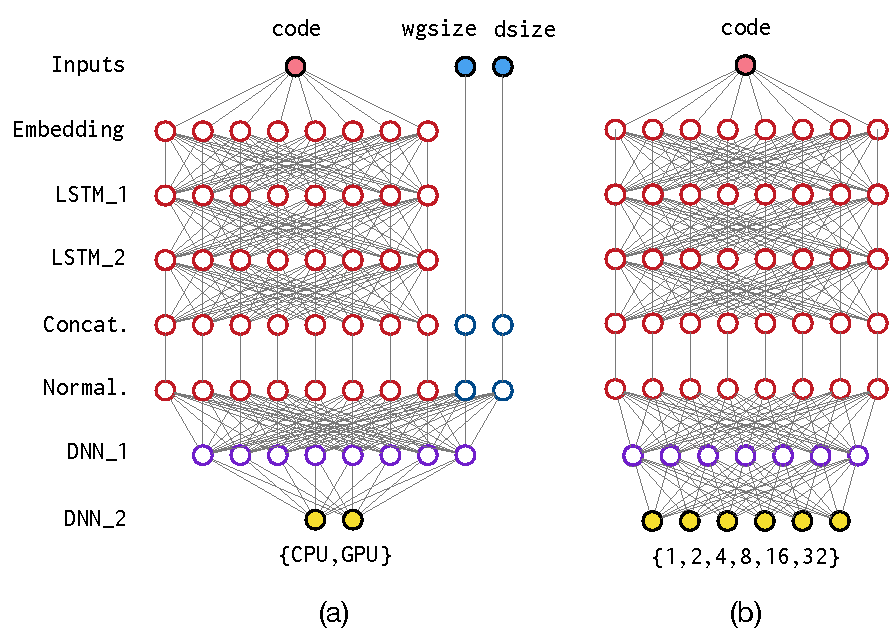
\includegraphics[width=\columnwidth]{img/nn} %
  \caption[DeepTune artificial neural networks]{%
    DeepTune artificial neural networks, configured for (a) heterogeneous mapping, and (b) thread coarsening factor. The design stays almost the same regardless of the optimisation problem. The only changes are the extra input for (a) and size of the output layers.%
  }%
  \label{fig:nn}
\end{figure}



\subsection{Case Study B: OpenCL Thread Coarsening Factor} \label{subsec:case-study-b}

\begin{figure}
  \centering %
  \subfloat[Magni \emph{et al.\ }cascading binary model.]{%
    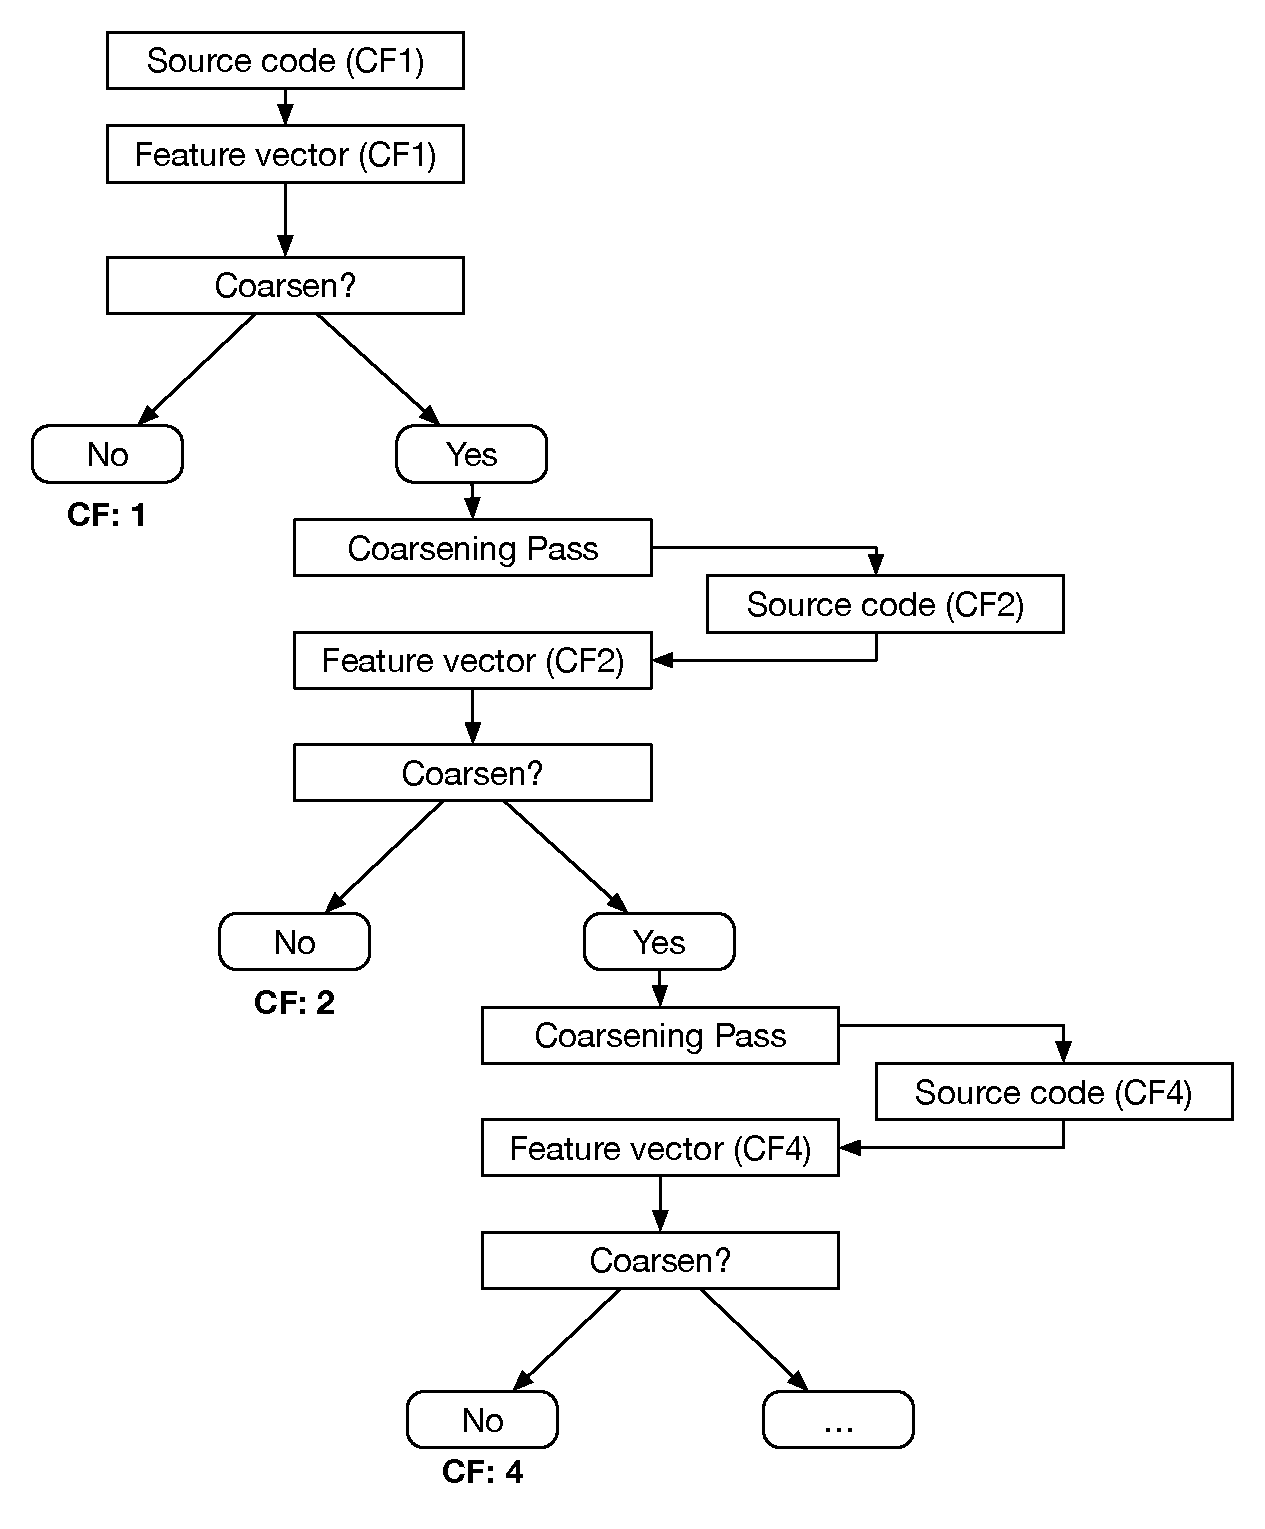
\includegraphics[width=.85\columnwidth]{img/cf-magni}%
    \label{fig:cf-magni}
  }\\*%
  \subfloat[Our approach.]{%
      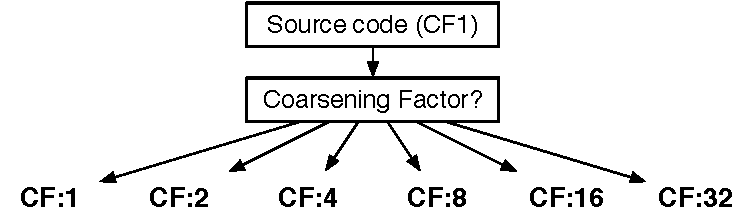
\includegraphics[width=.65\columnwidth]{img/cf-deeptune}%
      \label{fig:cf-deeptune}
  }%
  \caption{%
      Two approaches for predicting coarsening factor (CF) of OpenCL kernels.
      Magni \emph{et al.\ }reduce the multi-label classification problem to a
      series of binary decisions, by iteratively applying the optimization and
      computing new feature vectors. Our approach simply predicts the coarsening
      factor directly from the source code.%
  }
  \label{fig:cascading-nn}
\end{figure}


Thread coarsening is an optimization for parallel programs in which the operations of two or more threads are fused together. This optimization can prove beneficial on certain combinations of programs and architectures, for example programs with a large potential for Instruction Level Parallelism on Very Long Instruction Word architectures.

\subsubsection{State-of-the-art} Magni \emph{et al.\ }present a predictive model for OpenCL thread coarsening in~\cite{Magni2014}. They implement an iterative heuristic which determines whether a given program would benefit from coarsening. If yes, then the program is coarsened, and the process repeats, allowing further coarsening. In this manner, the problem is reduced from a multi-label classification problem into a series of binary decisions, shown in Figure~\ref{fig:cf-magni}. They select from one of six possible coarsening factors: $(1, 2, 4, 8, 16, 32)$, divided into 5 binary choices.

\begin{table}
  \rowcolors{2}{gray!25}{white}
  \centering%
    \begin{tabular}{| l l |}
      \hline
      \rowcolor{gray!50}
      \textbf{Name} & \textbf{Description} \\
      \hline
      \texttt{BasicBlocks} & \#.\ basic blocks \\
      \texttt{Branches} & \#.\ branches \\
      \texttt{DivInsts} & \#.\ divergent instructions \\
      \texttt{DivRegionInsts} & \#.\ instructions in divergent regions \\
      \texttt{DivRegionInstsRatio} & \#.\ instr. in divergent regions / total instructions \\
      \texttt{DivRegions} & \#.\ divergent regions \\
      \texttt{TotInsts} & \#.\ instructions \\
      \texttt{FPInsts} & \#.\ floating point instructions \\
      \texttt{ILP} & average ILP / basic block \\
      \texttt{Int/FP Inst Ratio} & \#.\ branches \\
      \texttt{IntInsts} & \#.\ integer instructions \\
      \texttt{MathFunctions} & \#.\ match builtin functions \\
      \texttt{MLP} & average MLP / basic block \\
      \texttt{Loads} & \#.\ loads \\
      \texttt{Stores} & \#.\ stores \\
      \texttt{UniformLoads} & \#.\ loads unaffected by coarsening direction \\
      \texttt{Barriers} & \#.\ barriers \\
      \hline
    \end{tabular}%
    \label{tab:features-pact14-raw}%
  \caption[\emph{Magni et al.\ }features for predicting thread coarsening]{%
    Candidate features used by \emph{Magni et al.\ }for predicting thread
    coarsening. From these values, they compute relative deltas for each
    iteration of coarsening, then use PCA for selection.%
  }%
  \label{tab:magni-features} %
\end{table}


\subsubsection{Expert Chosen Features} Magni \emph{et al.\ }followed a very comprehensive feature engineering process. 17 candidate features were assembled from previous studies of performance counters and computed theoretical values~\cite{Magni2,Sim2012}. For each candidate feature they compute its coarsening \emph{delta}, reflecting the change in each feature value caused by coarsening: $f_{\Delta} = (f_{after} - f_{before}) / f_{before}$, adding it to the feature set. Then they use Principle Component Analysis (PCA) on the 34 candidates and selected the first 7 principle components, accounting for 95\% of variance in the space.

\subsubsection{Experimental Setup} We replicate the experimental setup of Magni \emph{et al.}~\cite{Magni2014}. The thread coarsening optimization is evaluated on 17 programs, listed in Table~\ref{tab:pact-benchmarks}. Four different GPU architectures are used, listed in Table~\ref{tab:pact-platforms}.

\subsubsection{DeepTune Configuration} Figure~\ref{fig:nn}b shows the neural network configuration. We use the OpenCL kernel as input, and directly predict the coarsening factor.

\subsubsection{Model Evaluation} Compared to Case Study A, the size of the evaluation is small. We use \emph{leave-one-out cross-validation} to evaluate the models. For each program, a model is trained on data from all other programs and used to predict the coarsening factor of the excluded program.

Because~\cite{Magni2014} does not describe the parameters of the neural network, we perform an additional, \emph{nested} cross-validation process to find the optimal model parameters. For every program in the training set, we evaluate 48 combinations of network parameters. We select the best performing configuration from these 768 results to train a model for prediction on the excluded program. This nested cross-validation is repeated for each of the training sets. We do not perform this tuning of hyper-parameters for DeepTune.


\subsection{Comparison of Case Studies}

\begin{table}
  \centering
  \rowcolors{2}{white}{gray!25}
  \begin{tabular}{| l r r | r r |}
    \hline
    \rowcolor{gray!50}
    & \multicolumn{2}{c}{\textbf{\#.\ neurons}} & \multicolumn{2}{c}{\textbf{\#.\ parameters}} \\
    \rowcolor{gray!50}
    & \textbf{HM} & \textbf{CF} & \textbf{HM} & \textbf{CF} \\
    \hline
    \textbf{Embedding} & 64 & 64 & ,256 & 8,256 \\
    \textbf{LSTM\_1} & 64 & 64 & 33,024 & 33,024 \\
    \textbf{LSTM\_2} & 64 & 64 & 33,024 & 33,024 \\
    \textbf{Concatenate} & 64 + 2 & - & - & - \\
    \textbf{Batch Normalisation} & 66 & 64 & 264 & 256 \\
    \textbf{DNN\_1} & 32 & 32 & 2,144 & 2,080 \\
    \textbf{DNN\_2} & 2 & 6 & 66 & 198 \\
    \hline
    \textbf{Total} & & & 76,778 & 76,838 \\
    \hline
  \end{tabular}
  \caption[DeepTune model parameters]{%
    The size and number of parameters of the DeepTune components of
    Figure~\ref{fig:nn}, configured for heterogeneous mapping (HM) and
    coarsening factor (CF).%
  }
  \label{tab:nn-size}
\end{table}


For the two different optimization heuristics, the authors arrived at very different predictive model designs, with very different features. By contrast, we take exactly the same approach for both problems. None of DeepTune's parameters were tuned for the case studies presented above. Their settings represent conservative choices expected to work reasonably well for most scenarios.

Table~\ref{tab:nn-size} shows the similarity of our models. The only difference between our network design is the auxiliary inputs for Case Study A and the different number of optimization decisions. The differences between DeepTune configurations is only two lines of code: the first, adding the two auxiliary inputs; the second, increasing the size of the output layer for Case Study B from two neurons to six. The description of these differences is larger than the differences themselves.
